%!TEX root = ..\Master.tex

\subsection{Support Vector Machines}

e.g. decision function, support vectors, soft margins, kernel trick.\\

Introtext\\

It is supervised.

Compared to neural network and logistic regression, it sometimes gives a cleaner and more powerful way of learning complex non-linear functions.

Hard margin (linear): Finds the line that seperates the data with the largest margin.

Soft margin (linear): Finds the (TODO: Curve?) that seperates the data with the largest margin.

\begin{figure}[H]
\centering
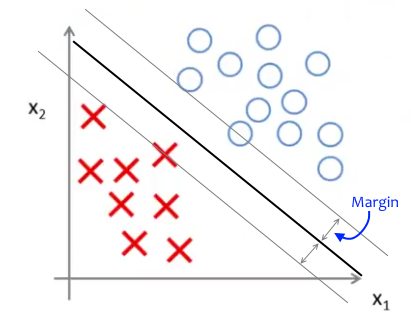
\includegraphics{billeder/svm-margin}
\caption{TODO}
\label{fig:svm-margin}
\end{figure}
The figure is only true when $C = \frac{1}{\lambda}$ (regularization term) is very large.

TODO: hard margin vs soft margin. 
TODO: Kernels.
Math\\

How we use it or why we don't use it\\

Intermediate result\\

%------------------------------------------------